\documentclass[11pt]{article}

\usepackage[margin=1.05in]{geometry}
\usepackage[T1]{fontenc}
\usepackage{mathpazo}
\usepackage[scaled=0.92]{helvet}
\usepackage{courier}
\usepackage{amsmath,amssymb,mathtools,bm}
\usepackage{booktabs,array,multirow}
\usepackage{enumitem}
\usepackage{xcolor}
\usepackage{graphicx}
\usepackage{tikz}
\usepackage{tcolorbox}
\usepackage{titlesec}
\usepackage{caption}
\usepackage{microtype}
\usepackage{needspace}
\usepackage[hidelinks]{hyperref}

\usetikzlibrary{positioning,arrows.meta,calc}
\tcbuselibrary{skins,breakable}

% ---------------------------------------------------------------- palette
\definecolor{navy}{RGB}{25,55,92}
\definecolor{muted}{RGB}{90,96,105}
\definecolor{rule}{RGB}{200,201,196}
\definecolor{okgreen}{RGB}{0,110,60}
\definecolor{specblue}{RGB}{42,120,214}
\definecolor{newmag}{RGB}{160,45,120}
\definecolor{openamber}{RGB}{170,110,0}
\definecolor{limred}{RGB}{175,45,45}
\definecolor{tint}{RGB}{248,248,246}
\definecolor{lg}{RGB}{175,177,172}

% ---------------------------------------------------------------- headings
\titleformat{\section}{\normalfont\sffamily\large\bfseries\color{navy}}{\thesection}{0.7em}{}
\titleformat{\subsection}{\normalfont\sffamily\normalsize\bfseries\color{navy}}{\thesubsection}{0.6em}{}
\titleformat{\part}[display]
  {\normalfont\sffamily\Large\bfseries\color{navy}\filcenter}
  {\MakeUppercase{\partname~\thepart}}{0.4em}{}
\titlespacing*{\section}{0pt}{1.5em}{0.6em}
\titlespacing*{\subsection}{0pt}{1.2em}{0.45em}

% ---------------------------------------------------------------- macros
\newcommand{\R}{\mathbb{R}}
\newcommand{\Prob}{\mathbb{P}}
\newcommand{\Ind}{\mathbf{1}}
\newcommand{\dhat}{\hat{d}}
\newcommand{\pihat}{\hat{\pi}}
\newcommand{\nhat}{\hat{n}}
\newcommand{\chat}{\hat{c}}
\newcommand{\that}{\hat{t}}
\newcommand{\Dhat}{\hat{\Delta}}

\newcommand{\provtag}[2]{{\footnotesize\sffamily\textcolor{#1}{[#2]}}}
\newcommand{\VALID}{\provtag{okgreen}{VALIDATED}}
\newcommand{\SPEC}{\provtag{specblue}{SPECIFIED}}
\newcommand{\NEWT}{\provtag{newmag}{NEW}}
\newcommand{\OPENT}{\provtag{openamber}{OPEN}}
\newcommand{\LIMIT}{\provtag{limred}{LIMIT}}

\newcommand{\why}[1]{\par\smallskip\noindent\textcolor{muted}{\small\itshape #1}\par\smallskip}

\newtcolorbox{claimbox}[1][]{
  enhanced, breakable, colback=tint, colframe=navy, boxrule=0pt,
  leftrule=2.5pt, arc=0pt, outer arc=0pt,
  left=12pt, right=12pt, top=9pt, bottom=9pt, #1}

\newtcolorbox{resultbox}[1][]{
  enhanced, breakable, colback=okgreen!4, colframe=okgreen!55, boxrule=0pt,
  leftrule=2.5pt, arc=0pt, outer arc=0pt,
  left=12pt, right=12pt, top=9pt, bottom=9pt, #1}

\newtcolorbox{limitbox}[1][]{
  enhanced, breakable, colback=limred!4, colframe=limred!55, boxrule=0pt,
  leftrule=2.5pt, arc=0pt, outer arc=0pt,
  left=12pt, right=12pt, top=9pt, bottom=9pt, #1}

\newtcolorbox{codebox}[1][]{
  enhanced, breakable, colback=tint, colframe=rule, boxrule=0.5pt,
  arc=2pt, left=10pt, right=8pt, top=7pt, bottom=7pt,
  fontupper=\footnotesize\ttfamily, #1}

\newtcolorbox{notebox}[1][]{
  enhanced, breakable, colback=white, colframe=rule, boxrule=0.5pt,
  arc=2pt, left=10pt, right=10pt, top=7pt, bottom=7pt,
  fontupper=\small, #1}

\captionsetup{font=small,labelfont={sf,bf,color=navy}}
\setlist[itemize]{leftmargin=1.3em,itemsep=2pt,topsep=4pt}
\setlist[enumerate]{leftmargin=1.6em,itemsep=2pt,topsep=4pt}
\renewcommand{\arraystretch}{1.15}

\hypersetup{pdfauthor={Robert Romani}}


\hypersetup{
  pdftitle={Experimental Report: Distance, Orientation, and Scaffold Characterisation},
  pdfsubject={Runs of 13 August 2026},
}

\title{\textcolor{navy}{\sffamily Experimental Report}\\[6pt]
\large\normalfont Distance recovery, orientation recovery, and scaffold characterisation\\
\normalsize\textcolor{muted}{Runs of 13 August 2026}}
\author{Robert Romani}
\date{August 13, 2026}

\begin{document}
\maketitle

\begin{abstract}
\noindent Three experiments, run and reported against predictions stated beforehand. Together
they establish the two links that carry the scientific claim of
\texttt{boundary\char`_recovery\char`_v5} --- that the \emph{distance} to a hidden routing boundary
and its \emph{direction} are both recoverable from query-only observations --- and they
characterise the real adversarial target the method is aimed at.

\medskip
\noindent Of seven predictions, four were confirmed and three falsified. The falsifications were
the more useful half: one inverted a design axis of the next experiment, one moved the mixture
likelihood-ratio test onto the critical path, and one retired the explicit falsification
condition that could have sunk the whole approach.
\end{abstract}

\noindent\textbf{\sffamily\small\textcolor{navy}{Provenance tags.}}
\smallskip

{\small
\begin{tabular}{@{}ll@{}}
\VALID & measured against ground truth\\
\SPEC & designed, not yet run\\
\NEWT & new finding from these runs\\
\OPENT & acknowledged gap\\
\LIMIT & structural impossibility\\
\end{tabular}}

\vspace{0.5em}

\section{Summary}

\begin{table}[h]
\small
\begin{tabular}{@{}cp{0.34\textwidth}p{0.46\textwidth}@{}}
\toprule
\textbf{\sffamily \#} & \textbf{\sffamily Prediction, as stated} & \textbf{\sffamily Outcome}\\
\midrule
E1-a & $\dhat = -\sigma\Phi^{-1}(\pihat)$ recovers true distance
     & \textbf{CONFIRMED.} $r = 0.9958$, median relative error $-0.92\%$.\\
E1-b & implied distance is constant across rungs for a gate and wanders for a smooth confound
     & \textbf{CONFIRMED.} CV $0.098$ against $0.56$--$1.24$.\\
E2-a & misassignment attenuates but does not rotate: bias $\approx 0$, variance up
     & \textbf{CONFIRMED.} Bias not significant in \textbf{0 of 20} cells.\\
E2-b & orientation error is U-shaped in $\pi$, optimum near $0.15$--$0.30$
     & \textbf{FALSIFIED.} Monotone \emph{increasing}; low $\pi$ is best.\\
S-1 & the OOD detector calls $>80\%$ of our probes real
    & \textbf{CONFIRMED on 3 of 4} (0.98 / 0.91 / 0.83 against 0.000 for LIME).
      Missed on Communities \& Crime.\\
S-2 & the scaffold's $\Delta/\sigma_{\text{resid}}$ exceeds $2.5$
    & \textbf{FALSIFIED.} $1.60$ / $1.88$ / $1.95$ --- at the dip's floor.\\
S-3 & retention falls below $\rho_{\min}$; the audit abstains on its own target
    & \textbf{FALSIFIED.} $\rho = 0.985$--$0.997$, zero anchors below threshold.\\
\bottomrule
\end{tabular}
\end{table}

\begin{claimbox}
\noindent\textbf{What the three experiments jointly establish.} From query access alone, at an
anchor near a hidden additive gate, both the \emph{distance} to the boundary and its
\emph{direction} are recoverable with quantified error; per-anchor direction error is pure
variance, so it pools away; and against the published adversarial target the probes are neither
recognised by its detector nor rejected by our own on-manifold filter.
\end{claimbox}

\part{Experiment 1 --- the distance estimator}

\section{Question}

A two-component fit at an anchor returns a mixing fraction $\pihat$: the share of probes that
landed on the far side of the gate. For a probe cloud $z \sim N(0,\sigma^2 I)$ and a unit normal
$n$, the signed projection $z^\top n$ is $N(0,\sigma^2)$, so crossing at distance $d$ occurs with
probability $\Phi(-d/\sigma)$. Read backwards,
\[
  \boxed{\;\dhat_s \;=\; -\sigma_s\,\Phi^{-1}(\pihat_s)\;}
\]
The crossing law itself is validated to three decimals (E1a, July). Using it as an
\emph{estimator} of distance to an unobservable boundary had never been tried.

\section{Design}

The registered 1-D known-regimes setting: gate at $x = 0.5$ with $\Delta = 0.30$, honest slope
$0.15$, ladder \texttt{geomspace(0.02, 0.2, 3)}, $m = 1000$ probes per rung. The stored
\texttt{sim1d\char`_anchors.csv} keeps only a \emph{median} of $\pihat$ across scales, so the
inversion was not testable from it; the experiment reruns the protocol recording $\pihat$ per
scale.

Orientation is query-only: the anchor's own response says which mixture component it sits in,
and the crossing mass is the other one. Six models --- gated, honest, a kink control, and three
Gaussian-process nulls with lengthscales above and below the ladder top --- across a $10\times$
noise sweep, 3{,}218 anchor-by-rung rows.

Two guards, both computable without ground truth: the dip fires under Bonferroni, and
$\pihat \in [0.05, 0.50]$.

\section{Results}

\begin{resultbox}
\noindent $\mathrm{corr}(\dhat, d_{\text{true}}) = \mathbf{0.9958}$ \ ($n = 217$) \quad$\cdot$\quad
median relative error $\mathbf{-0.92\%}$ \quad$\cdot$\quad median absolute error $0.0031$

\smallskip
\noindent Tracks correctly across every bin from $d = 0.012$ to $0.251$, and is flat across a
$10\times$ noise sweep: median absolute error $0.0029 / 0.0031 / 0.0027$ at
$\tau = 0.005 / 0.02 / 0.05$.
\end{resultbox}

\noindent Relative error degrades close to the boundary --- $3.3\%$ beyond $d = 0.1$, $5.0\%$ at
$0.05$--$0.1$, $26\%$ below $0.01$ --- where the \emph{absolute} error is still ${\sim}0.003$ and
only the denominator is small. Report absolute error near the boundary.

\paragraph{The second invariance.} \NEWT\ For a planar boundary at fixed distance, $\dhat_s$
should not depend on the rung. It does not for a gate, and does for a smooth confound:

\begin{table}[h]
\small\centering
\begin{tabular}{@{}lcc@{}}
\toprule
\textbf{\sffamily Model} & \textbf{\sffamily median CV of} $\dhat$ & \textbf{\sffamily fire rate}\\
\midrule
\textbf{gated} & \textbf{0.098} \ (0.074 at $\tau = 0.02$) & 0.678\\
GP null, $\ell = 0.05$, $A = 0.10$ & 0.557 & 0.397\\
GP null, $\ell = 0.05$, $A = 0.20$ & 1.042 & 0.114\\
kink control & 1.241 & 0.023\\
honest & --- & \textbf{0.000}\\
GP null, $\ell = 0.30$ (above ladder top) & --- & \textbf{0.000}\\
\bottomrule
\end{tabular}
\end{table}

\noindent At $\mathrm{CV} < 0.15$: 56\% of gates retained, 93\% of confounders rejected. As a
standalone filter that is expensive; its value is as one of three orthogonal checks, and the
operating point should be set once the full pipeline exists.

\begin{figure}[!ht]
\centering
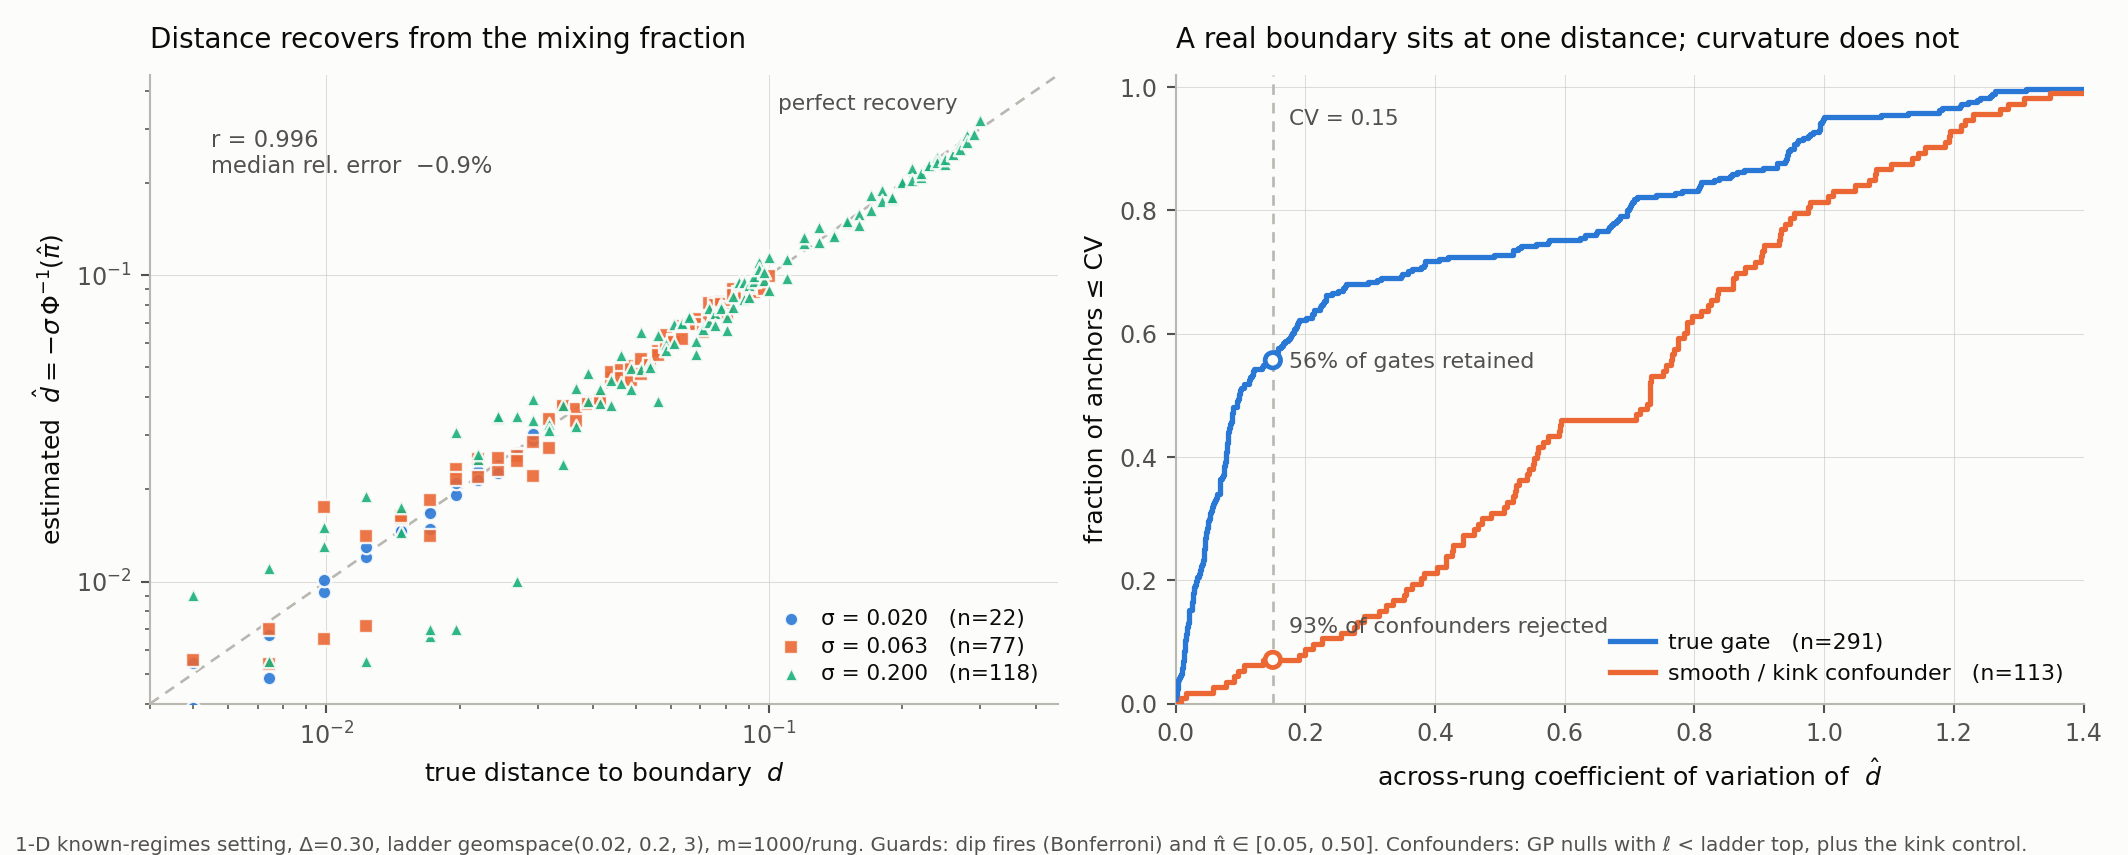
\includegraphics[width=\textwidth]{fig_distance_estimator.png}
\caption{\textbf{Left:} recovered against true distance, by probe scale. \textbf{Right:}
across-rung constancy of $\dhat$ separates a gate from smooth and kink confounders.}
\end{figure}

\section{What this did not establish}

The estimate is \textbf{conditional on detection.} Without the dip guard, anchors beyond the
ladder top return confident nonsense --- true $0.277$ against estimated $0.141$, with enormous
spread --- because $\pihat$ there is not a crossing fraction at all. The guard is query-only, so
the conditioning is legitimate, but it belongs in the claim.

And this ran the \textbf{naive} protocol: 1-D, ambient Gaussian probes, no tangent frame, no
trimming, no density filter. It validates the inversion, not the inversion inside the pipeline.
\OPENT

\part{Experiment 2 --- the orientation estimator}

\section{Question}

The Stage-3 separability guard fits a linear classifier on (probe coordinates, mixture
responsibilities). Its decision boundary, lifted through the tangent frame, is an estimate of the
gate's normal --- so test and recovery are the same computation. The concern this had to answer:
\textbf{responsibilities are estimated, not true branch labels}, so the chain
\[
  \text{mixture misassignment} \;\to\; \text{classifier label noise} \;\to\; \text{bias in } \nhat
\]
could dominate everything else near weak separation.

\begin{claimbox}
\noindent The right figure of merit is not mean error but the \textbf{bias/variance split}.
Independent unbiased errors shrink as $1/\sqrt{N}$ under pooling --- $40^\circ$ per anchor
becomes ${\sim}4^\circ$ at $N=100$. A systematic $5^\circ$ rotation is still $5^\circ$ after 200
anchors, and propagates straight into $\that = \chat/\nhat_i$.
\end{claimbox}

\section{Design}

Intrinsic $d = 2$ in ambient $D = 20$, flat manifold, planted hyperplane, frame supplied
(Stage 0 deferred). The true normal is drawn per anchor so no coordinate is privileged; error is
$\angle(\nhat, n)$ modulo sign. 200 anchors per cell over a $\Delta/\tau \times \pi$ grid,
$m = 1000$ probes per anchor, 4{,}000 anchors total.

\textbf{The instrument is an oracle contrast:} fit the discriminant twice at each anchor --- once
on estimated responsibilities, once on the \emph{true} branch labels, which exist by construction
--- and difference the orientation errors. The oracle arm is the variance floor; the gap is the
misassignment cost.

\section{Results}

\begin{resultbox}
\noindent\textbf{Misassignment costs variance, not bias.} Mean signed rotation per cell: the
oracle arm lies in $[-0.35^\circ, +0.27^\circ]$; the estimated-responsibility arm lies in
$[-6.6^\circ, +5.9^\circ]$ and is \textbf{not significant at 95\% in any of the 20 cells}.

\smallskip
\noindent Pooled orientation error falls as $1/\sqrt{N}$: at $\pi = 0.05$, from $6.8^\circ$ to
$0.9^\circ$ between $N = 1$ and $N = 100$ at $\Delta/\tau = 2.5$, and $20.4^\circ \to 1.8^\circ$
at $\Delta/\tau = 1.5$ --- below the dip's floor entirely.
\end{resultbox}

\paragraph{Why there is no rotation.} The result has a mechanism rather than being empirical
luck. For $z \sim N(0,\sigma^2 I)$ and a half-space boundary, both class-conditional means of $z$
lie \emph{exactly} along $n$: the components orthogonal to $n$ are independent of $z^\top n$, so
their conditional means vanish. Since the responsibilities are a function of the
one-dimensional residual, and the residual is a function of $z^\top n$, the responsibilities are
a function of $z^\top n$ alone --- so corrupted labels attenuate the separation without turning
it.

\paragraph{Prediction E2-b falsified, and in the opposite direction.} Orientation error is
\textbf{monotone increasing} in $\pi$, not U-shaped. Per-anchor standard deviation at
$\Delta/\tau = 5$ runs $3.9^\circ$ at $\pi = 0.05$ to $47.5^\circ$ at $\pi = 0.50$. The reasoning
behind the prediction --- few crossers means a noisy discriminant --- was wrong because the
crossers sit further out along the normal, and the separation of class-conditional means
\emph{rises} as $\pi$ falls:

\begin{center}\small
\begin{tabular}{@{}lccccc@{}}
\toprule
$\pi$ & 0.05 & 0.10 & 0.20 & 0.35 & 0.50\\
\midrule
mean separation along $n$ & $2.17\sigma$ & $1.95\sigma$ & $1.75\sigma$ & $1.63\sigma$ & $1.60\sigma$\\
\bottomrule
\end{tabular}
\end{center}

\noindent At $\pi \to 0.5$ there is additionally no majority branch for LTS to trim toward.

\begin{figure}[!ht]
\centering
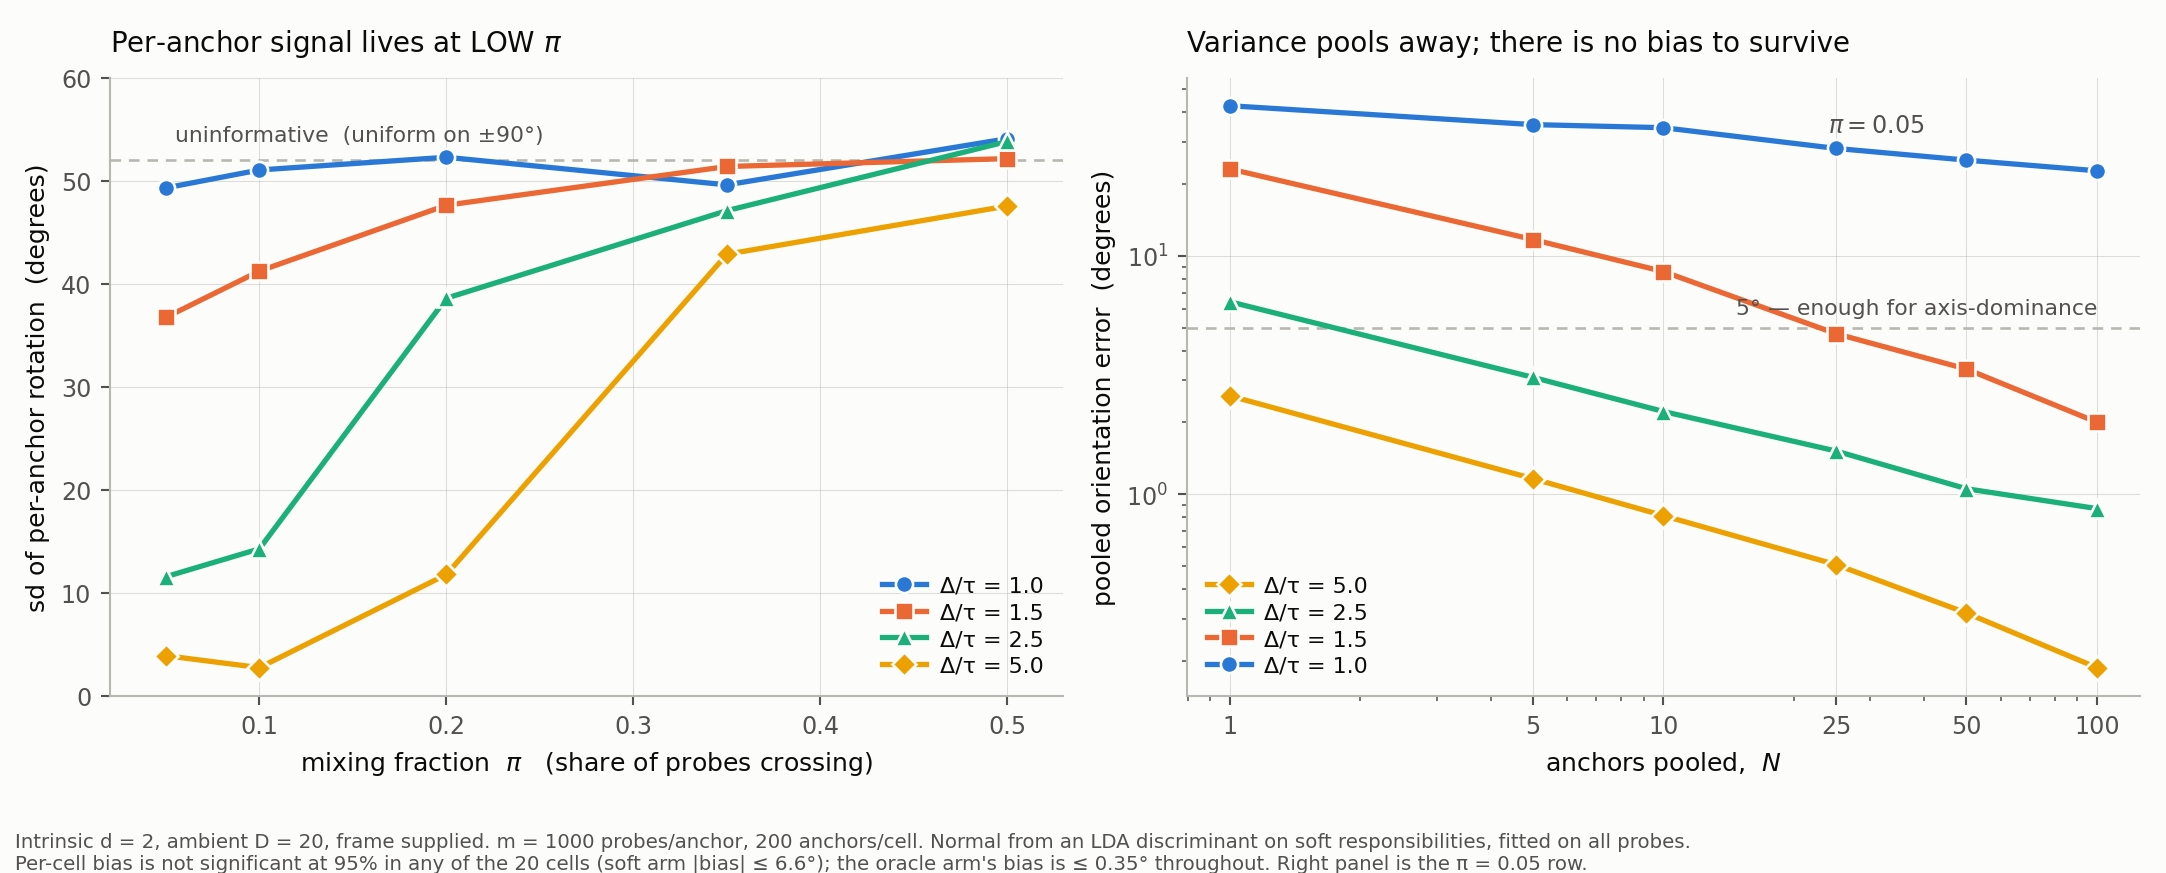
\includegraphics[width=\textwidth]{fig_normal_estimator.png}
\caption{\textbf{Left:} per-anchor information against the mixing fraction; $52^\circ$ is what
uniformly random directions give. \textbf{Right:} pooled error against anchors, at $\pi = 0.05$.}
\end{figure}

\section{Consequences for the method} \NEWT

\begin{itemize}
\item \textbf{Fit the discriminant on all probes, not the LTS inlier set} --- $5.8^\circ$ against
$21.9^\circ$ median error. The trim removes points that are predominantly the minority branch,
which is exactly the branch carrying the crossing signal. Trim for the \emph{mixture}; discard
the mask for the \emph{discriminant}.
\item \textbf{Soft responsibilities beat hard} $\gamma > 0.5$ \textbf{labels} --- $5.8^\circ$
against $7.6^\circ$.
\item \textbf{Useful anchors sit at low $\pi$}, i.e.\ $d/\sigma \in [1.28, 1.64]$. This inverts
Experiment P's distance axis, whose small values placed anchors close to the boundary. It also
agrees with the distance estimator, so one rung serves both.
\end{itemize}

\begin{limitbox}
\noindent\textbf{A no-information guard is now required.} Outside the operating region
($\Delta/\tau = 1.0$ at any $\pi$, or $\pi \gtrsim 0.35$) the per-anchor rotation has standard
deviation $\approx 52^\circ$ --- what uniformly random directions give. Pooling uninformative
\emph{axial} estimates does not converge to the truth and does not converge to nothing: the mean
direction of $N$ random axes is itself uniformly random, so the pooled estimate lands on an
arbitrary direction with an interval that \emph{tightens} around it. Pooling can be confidently
wrong in a way per-anchor abstention never is.
\end{limitbox}

\section{What this did not establish}

Intrinsic $d = 2$ only. The discriminant is a direction in $\R^{\hat d}$, so error should scale
with \emph{intrinsic} dimension; E1's dimension-independence result concerns \emph{ambient} $D$
and does not transfer. \OPENT

The pooled curve was simulated by averaging rotations measured \emph{relative to known truth}.
Real pooling has no reference and must find the mode; in $d=2$ with a common normal the variance
behaviour transfers, but the estimator itself and the offset $\chat$ remain untested. That is
Experiment P.

\part{Experiment 3 --- scaffold characterisation}

\section{Question}

Every power figure in the project is measured against gates we planted ourselves. The target is
the Slack et al.\ (AIES 2020) scaffolding attack: a biased $f$, an innocuous $\psi$, and a random
forest trained to separate real data from LIME-perturbed samples, routing between them.

Two measurements decide what the rest of the work is for. \textbf{S5}: what fraction of the
audit's own probes does the detector call real? LIME perturbs every feature ambiently with
$N(0,0.3)$; ours is isotropic inside a $\hat d$-dimensional tangent frame at the local geometric
scale --- a distribution the detector was never trained against. \textbf{S1}: what is the
scaffold's actual $\Delta/\sigma_{\text{resid}}$?

\section{Design}

Four targets: our geospatial housing scaffold, and COMPAS, German Credit and Communities \&
Crime through Slack's own \texttt{adversarial\char`_models}. 150 anchors per target, 400 probes
per anchor, frame and radius supplied by local PCA on the 60 nearest real points. Probes are
generated in standardised space and mapped back to raw units, because raw units are what the
detector sees. A radius sweep over $\{0.02 \dots 1.00\}\times$ the local $k$-NN scale turns S5
from a yes/no into a curve.

\section{Results}

\begin{table}[h]
\small\centering
\begin{tabular}{@{}lccccc@{}}
\toprule
\textbf{\sffamily Target} & \textbf{S5} audit & \textbf{S5} LIME & \textbf{S3} $\rho$
  & straddle rate & response values\\
\midrule
COMPAS & 0.980 & 0.000 & 0.997 & 0.013 & 1\\
German & 0.900 & 0.000 & 0.987 & 0.253 & 2\\
Housing & 0.860 & 0.000 & 0.996 & 0.473 & 400\\
Communities \& Crime & \textbf{0.001} & 0.000 & 0.985 & 0.007 & 2\\
\bottomrule
\end{tabular}
\end{table}

\noindent S4 (detector leakage on real points) is $0.000$ everywhere, and \textbf{no anchor on
any target} had $\rho$ below $\rho_{\min}$.

\begin{resultbox}
\noindent\textbf{The detector identifies 100\% of LIME's own perturbations and misses 83--98\% of
ours.} It was trained to recognise exactly one perturbation family and generalises to no other.

\smallskip
\noindent\textbf{Housing resolves to trichotomy regime (ii).} Across the radius sweep,
invisibility decays gently ($0.94 \to 0.83$) while the fraction of anchors whose ball straddles
the OOD boundary rises sharply ($0.10 \to 0.53$). Both conditions hold at once: at full $k$-NN
radius, 83\% of probes are invisible and about half of anchors reach the gate. COMPAS is regime
(i) --- invisible but never crossing. German is mixed, at 25\%.
\end{resultbox}

\paragraph{S-2 falsified, and it costs.} $\Delta/\sigma_{\text{resid}}$ is $1.60$ (COMPAS),
$1.88$ (German), $1.95$ (housing) --- not the predicted ${>}2.5$. The real scaffold sits
\emph{at} the dip's floor, where measured power is $0.000$, and inside the equal-variance LRT's
$0.42$--$0.54$ band. \textbf{The LRT is therefore no longer optional, and neither is pooling.}
Its threshold has never been calibrated through the pipeline; that moves onto the critical path.

\paragraph{S-3 falsified, and it is the good kind.} The explicit falsification condition --- that
the density filter abstains exactly where the signal lives --- did \emph{not} fire. Retention is
$0.985$--$0.997$ on every target with zero anchors below threshold. This was the single result
that could have invalidated the on-manifold approach against this target.

\begin{figure}[!ht]
\centering
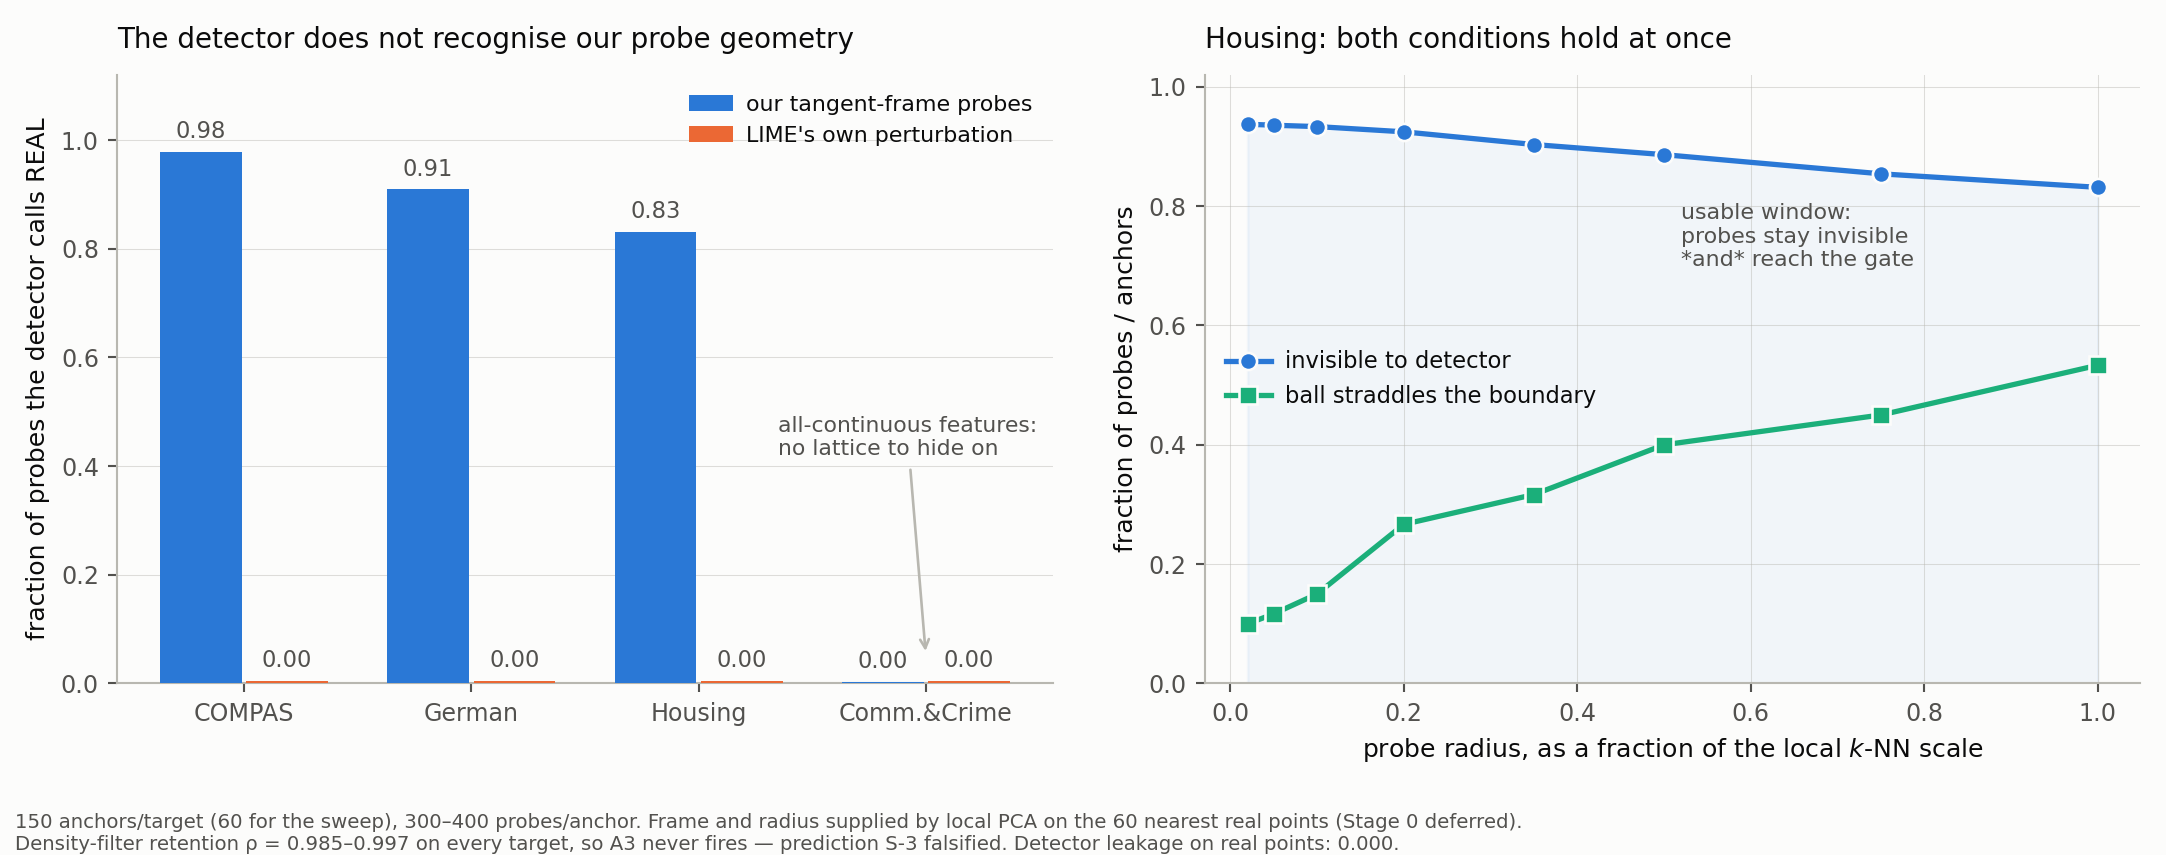
\includegraphics[width=\textwidth]{fig_s_experiment.png}
\caption{\textbf{Left:} probe visibility, ours against LIME's own. \textbf{Right:} the housing
operating window --- invisibility and boundary-crossing hold simultaneously.}
\end{figure}

\section{The Communities \& Crime miss}

Not a radius or frame artifact: visibility stays at $0.011$ with the dimension cap raised to 30,
and at $2\%$ of the $k$-NN radius. The mechanism appears to be a \textbf{lattice} effect. Adding
$10^{-3}$ of noise to a training point drops ``called real'' to $0.000 / 0.000 / 0.046$, while
genuinely held-out real points are still called real at ${\approx}1.0$ --- so the detector is not
memorising; it keys on off-grid movement in quantised coordinates.

Tangent-frame probing largely respects that grid, because low-dimensional local PCA on mixed
tabular data concentrates on the continuous directions. Off-lattice fraction: COMPAS $0.33$,
housing $0.62$, German $0.69$, \textbf{Communities \& Crime $0.96$} --- and its features are
nearly all continuous, so there is no grid to stay on.

\OPENT\ The ordering is right but this is not a clean single-factor account: German is $0.69$
off-lattice and still reaches $0.91$ visibility, so ambient dimension ($101$ against ${\le}29$)
is plausibly also at work. Directionally supported, not established.

\section{Two consequences}

\paragraph{A discrete-response Stage 3 is a confirmed prerequisite for the Slack datasets.} They
expose \textbf{one or two} distinct response values; housing gives 400. Stage 3 tests the shape
of a continuous residual distribution and does not apply to a binary response. Anticipated in the
31 July review; now measured.

\paragraph{A sharper claim is available.} Scaffolding attacks keyed on LIME's ambient Gaussian
perturbation are defeated by any probe family respecting the data's discrete structure ---
\emph{but not on all-continuous data}. That is a statement about the attack's scope, and
Communities \& Crime is the counterexample that makes it non-trivial.

\section{What this did not establish}

Experiment S showed the gate is \textbf{reachable}. It detected and recovered \emph{nothing}. The
end-to-end run against the housing scaffold is a separate piece of work and is now the clearest
route to the second deliverable.

\part{Consolidated}

\section{What changed in the method}

\begin{enumerate}
\item The distance estimator $\dhat = -\sigma\Phi^{-1}(\pihat)$ enters Stage 4. \NEWT
\item Across-rung constancy of $\dhat$ enters Stage 5 as a second invariance, orthogonal to the
$\Dhat$ scaling exponent. \NEWT
\item The discriminant fits on all probes, not the LTS inlier set. \NEWT
\item Anchor placement targets $\pi \le 0.10$; Experiment P's distance axis inverts. \NEWT
\item A no-information guard becomes part of Experiment P. \NEWT
\item LRT calibration through the pipeline moves onto the critical path, because the real target
sits at the dip's floor. \NEWT
\item The density-filter falsification condition is retired. \NEWT
\end{enumerate}

\section{Reproduction}

All seeded; all under \texttt{sim/} in \texttt{detect-recover-interpret}.

\begin{table}[h]
\small
\begin{tabular}{@{}lp{0.30\textwidth}p{0.36\textwidth}@{}}
\toprule
\textbf{\sffamily Experiment} & \textbf{\sffamily Script} & \textbf{\sffamily Outputs}\\
\midrule
1 --- distance & \texttt{exp\char`_distance\char`_estimator.py}
  & \texttt{distance\char`_estimator\char`_rows.csv} (3{,}218)\\
2 --- orientation & \texttt{exp\char`_normal\char`_estimator.py}
  & \texttt{normal\char`_estimator\char`_rows.csv} (4{,}000);
    \newline \texttt{normal\char`_estimator\char`_}\newline\texttt{probelog.csv.gz}\\
3 --- scaffold & \texttt{exp\char`_s\char`_scaffold.py}
    \texttt{exp\char`_s5\char`_radius.py}
  & \texttt{s\char`_experiment\char`_rows.csv}
    \texttt{s5\char`_radius\char`_sweep.csv}\\
\bottomrule
\end{tabular}
\end{table}

\noindent Figures are built by the matching \texttt{fig\char`_*.py}. Experiment 2's probe log
records per-probe coordinates, response, true label, fitted responsibility, trim mask and filter
mask, so any downstream arm --- oracle / soft / hard labels, trim on-off, filter on-off --- is
reconstructable as post-processing without a rerun. Experiment 3 requires the
\texttt{fooling-lime-shap} repository as a sibling checkout, plus \texttt{xgboost}; Experiment 1
uses \texttt{diptest} where available and a seeded Monte-Carlo null otherwise.

\section{Open items these runs created}

\begin{itemize}
\item Interval coverage on $(\nhat, \chat, \that)$ --- never measured, and it is what turns a
point estimate into a claim. \OPENT
\item Intrinsic-dimension scaling of orientation error. \OPENT
\item The no-information guard --- required, not yet designed. \OPENT
\item The lattice account of the Communities \& Crime miss --- directionally supported, not
established. \OPENT
\item A discrete-response Stage 3 variant, if the Slack datasets are to appear. \OPENT
\end{itemize}

\end{document}
